\documentclass[12pt,a4paper]{article}
\usepackage[UTF8]{ctex}
\usepackage{graphicx}
\usepackage{geometry}
\usepackage{ulem}
\usepackage{enumitem}
\usepackage{titlesec}
\usepackage{multicol}
\usepackage[export]{adjustbox}
\usepackage{amsmath}  % 推荐用于更好的数学排版
\usepackage[utf8]{inputenc}
\usepackage{CJKutf8}
\usepackage{fancyhdr}
\usepackage{lastpage}
\usepackage{ulem}
\usepackage{tabularx}
% 页眉页脚设置
\pagestyle{fancy}
\fancyhf{} % 清除所有页眉页脚
% 设置页眉内容
%-==========1. 填写从第二页开始 每页第一行的信息==========-
\fancyhead[C]{
    \makebox[4.5em][c]{实验名称：} \uline{\makebox[14em][c]{电路定理验证试验}} 
    \makebox[2.5em][c]{姓名：} \uline{\makebox[4em][c]{张三丰}} 
    \makebox[2.5em][c]{学号：} \uline{\makebox[5em][c]{1234567890}}
}%--------------------------------------------------------
\fancyfoot[C]{第 \thepage\ 页，共 \pageref{LastPage} 页}

% 取消页眉和页脚的下划线
\renewcommand{\headrulewidth}{0pt} % 页眉横线粗细设为0
\renewcommand{\footrulewidth}{0pt} % 页脚横线粗细设为0

% 调整页眉高度
\setlength{\headheight}{50pt}

% 设置plain样式（用于第一页）
\fancypagestyle{plain}{
    \fancyhf{} % 清除所有页眉页脚
    \renewcommand{\headrulewidth}{0pt} % 隐藏页眉横线
    \fancyfoot[C]{第 \thepage\ 页，共 \pageref{LastPage} 页} % 保留页脚
}
% 设置页面边距
\geometry{left=2.54cm,right=1.5cm,top=2.54cm,bottom=2.54cm}

% 设置正文字体大小为小四
\renewcommand{\normalsize}{\fontsize{12pt}{18pt}\selectfont}
% 设置章节格式
\titleformat{\section}{\fontsize{16pt}{24pt}\selectfont\bfseries}{\thesection}{1em}{} % 一级标题：三号
\titleformat{\subsection}{\fontsize{15pt}{22.5pt}\selectfont\bfseries}{\thesubsection}{1em}{} % 二级标题：小三

\begin{document}
\thispagestyle{plain}%第一页使用 plain 样式，而不是默认的 fancy 样式，第一页不再显示页眉
% 标题部分 - 两栏布局
\begin{multicols}{2}
    % 左栏：图片和实验报告标题
    % 左栏：使用空行创建前三行
    \noindent
    ~\\ % 第一行
    ~\\ % 第二行
    ~\\ % 第三行
    \hphantom{占位}% 使用空占位符
    \raisebox{-0.5\baselineskip}% 图片向下移动半行
    {
\includegraphics[width=1.85in,height=0.58in]{ZJU.jpg}}
    \hspace{.5em}% 图片和标题之间的间距
    \raisebox{0pt}[\height][0pt]% 标题底部对齐
    {\textbf{\fontsize{26pt}{30pt}\selectfont 实验报告}}
    
    \columnbreak % 换到右栏
    
    % 右栏：个人信息
    % 右栏：个人信息 - 靠右对齐 
%-==========2. 填写个人信息==========-
    \begin{flushright}
        \makebox[3em][l]{专业：} \uline{\makebox[9em][c]{信息与通信工程}} \\
        \makebox[3em][l]{姓名：} \uline{\makebox[9em][c]{张 三 丰}} \\
        \makebox[3em][l]{学号：} \uline{\makebox[9em][c]{1234567890}} \\
        \makebox[3em][l]{日期：} \uline{\makebox[9em][c]{2025年12月01日}} \\
        \makebox[3em][l]{地点：} \uline{\makebox[9em][c]{紫金港东四219}} \\
    \end{flushright}   
\end{multicols}
% 课程名称等信息（单栏）
%-==========3. 填写课程信息==========-
\noindent
课程名称： \uline{电子电路设计实验I} \hfill 指导老师： \uline{施红军、叶险峰、邓靖靖} \hfill 成绩： \uline{\hspace{3cm}} \\
实验名称： \uline{晶体管共射放大电路设计} \hfill 实验类型： \uline{设计类实验} \hfill 同组学生姓名： \uline{张三丰}
%-==========4. 正文开始==========-
\section*{一、实验目的}
%第一段内容：
验证基尔霍夫电压定理、基尔霍夫电流定理、叠加定理、诺顿定理、戴维南定理。
%-==========插入公式举例==========-
1. 举例如何添加公式：%记得在文档导言区添加数学支持包（通常 article 类已经包含了基本的数学支持）

（1）例一：公式居中独占一行%这是一个显示模式的数学公式，使用 \[ 和 \] 来创建单独一行的公式
\[
\sum_{m=1}^{M} v_m = 0
\]

（2）例二：在文本中添加公式

基尔霍夫电压定律$\sum_{m=1}^{M} v_m = 0$，该式表示在任一回路中电压代数和为零。%如果需要在文本内插入公式，可以使用。

（3）例三：这是添加了编号的公式：%如果需要在公式中添加编号，可以使用 equation 环境：
\begin{equation}
\sum_{m=1}^{M} v_m = 0
\end{equation}

2. 插入表格举例：有不懂的地方可以问Deepseek，逐步向Deepseek提出要修改的要求，它会为你修改代码的。
%-==========插入表格举例==========-
\begin{table}[ht!]
\footnotesize
\caption{\normalsize 95\% Confidence interval of penalty for the approximations and heuristics with $\rho=0.5$ } 
\centering  
\renewcommand{\arraystretch}{1.1}
\begin{tabular}{*{8}{l}} 
\hline\hline   
&$T=10$ &$T=30$ &$T=100$ &$T=300$ &$T=1000$ &$T=3000$ &$T=10000$  \\ 
\hline
$S_m$ & [0.13, 0.56]& [0.22, 0.79]& [0.18, 0.90]& [0.35, 0.92]& [0.11, 0.73]& [0.44, 0.87]& [0.06, 0.78]\\
$S_n$ & [0.28, 0.74]& [0.09, 0.45]& [0.31, 0.59]& [0.42, 0.97]& [0.15, 0.67]& [0.12, 0.76]& [0.08, 0.54]\\
$S_l$ & [0.07, 0.62]& [0.36, 0.88]& [0.05, 0.70]& [0.29, 0.61]& [0.14, 0.73]& [0.19, 0.82]& [0.27, 0.91]\\
$S_{log}$ & [0.18, 0.69]& [0.22, 0.81]& [0.15, 0.65]& [0.10, 0.58]& [0.25, 0.71]& [0.07, 0.55]& [0.04, 0.62]\\
$S_c$ & [0.09, 0.77]& [0.38, 0.79]& [0.24, 0.60]& [0.32, 0.89]& [0.28, 0.66]& [0.15, 0.84]& [0.22, 0.59]\\
$S_g$ & [0.05, 0.42]& [0.26, 0.73]& [0.33, 0.86]& [0.17, 0.69]& [0.30, 0.90]& [0.09, 0.78]& [0.14, 0.83]\\
\hline  
    \end{tabular}
    \label{table:summary05-CI}
\end{table}

3.举例如何插入图片
%-==========插入图片举例==========-
\begin{figure}[h]
    \centering
    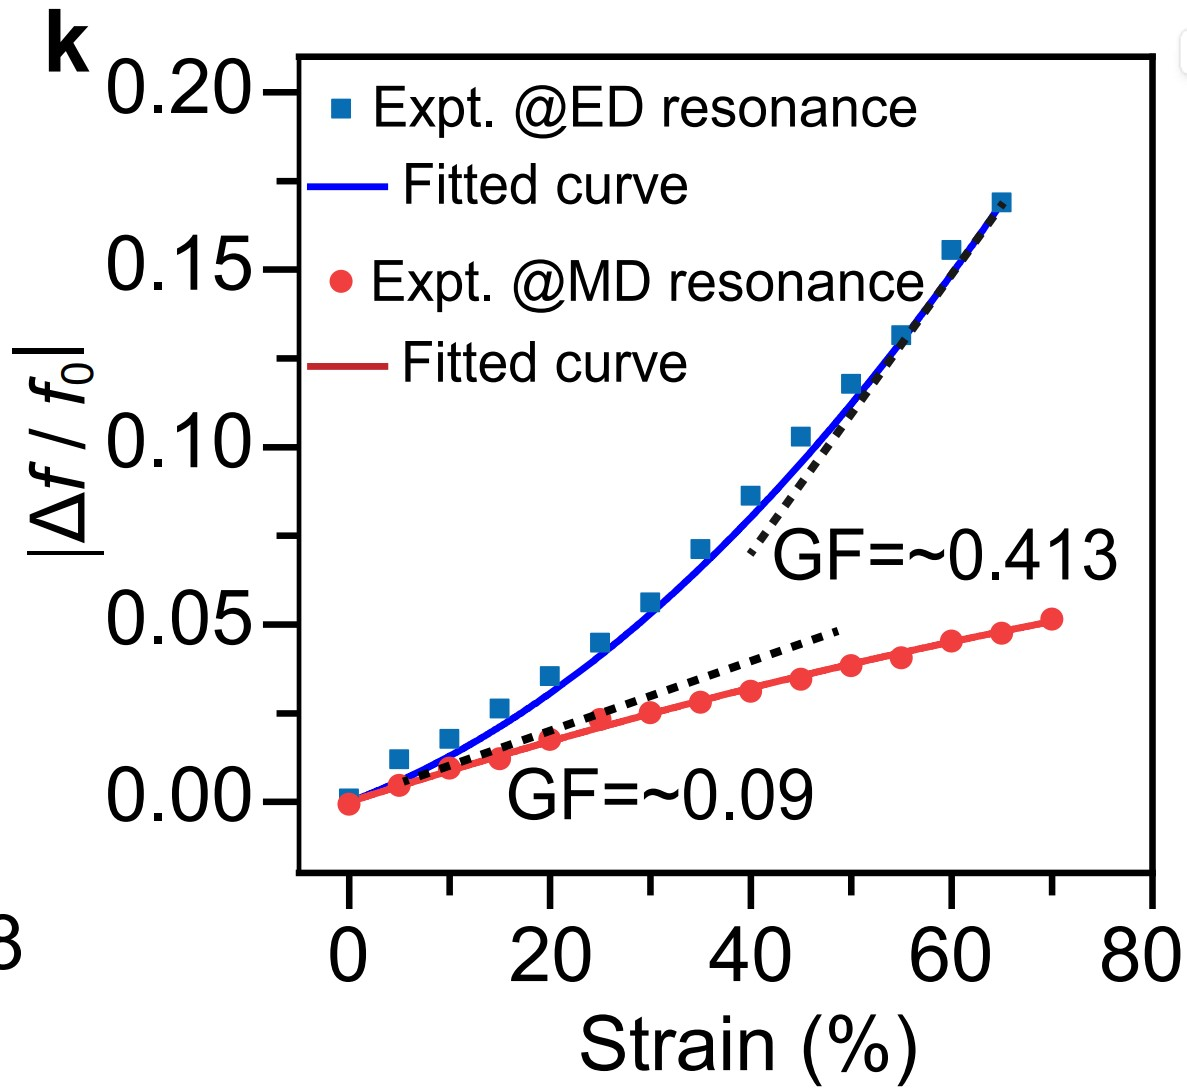
\includegraphics[width=0.4\textwidth, height=0.2\textheight]{ZJU2.jpg}
    \caption{电场和磁场谐振}
    \label{fig:1.1}
\end{figure}

如图\ref{fig:1.1}所示，图中。。。。。。。。。
\section*{二、实验任务与要求}
。。。。。

\section*{三、实验原理}
。。。。。

\section*{四、实验方案设计与参数计算}
\subsection*{4.1 实验方案总体设计}
。。。。。

\subsection*{4.2 各功能电路设计与计算}
。。。。。

\subsection*{4.3 完整的实验电路}
。。。。。

\section*{五、实验仪器设备}
。。。。。

\section*{六、实验步骤、调试过程、实验数据记录}
。。。。。

\section*{七、数据分析与讨论}
。。。。。

\section*{八、结论}
。。。。。

\section*{九、心得与体会}
。。。。。

\section*{十、思考题}
1. 题目内容

答：。。。。。

2.题目内容

答：。。。。。。。

3.题目内容

答：。。。。。。

\end{document}